\chapter{The Meeting}

After Mercédès had left Monte Cristo, he fell into profound gloom.
Around him and within him the flight of thought seemed to have stopped;
his energetic mind slumbered, as the body does after extreme fatigue.

“What?” said he to himself, while the lamp and the wax lights were
nearly burnt out, and the servants were waiting impatiently in the
anteroom; “what? this edifice which I have been so long preparing,
which I have reared with so much care and toil, is to be crushed by a
single touch, a word, a breath! Yes, this self, of whom I thought so
much, of whom I was so proud, who had appeared so worthless in the
dungeons of the Château d’If, and whom I had succeeded in making so
great, will be but a lump of clay tomorrow. Alas, it is not the death
of the body I regret; for is not the destruction of the vital
principle, the repose to which everything is tending, to which every
unhappy being aspires,—is not this the repose of matter after which I
so long sighed, and which I was seeking to attain by the painful
process of starvation when Faria appeared in my dungeon? What is death
for me? One step farther into rest,—two, perhaps, into silence. No, it
is not existence, then, that I regret, but the ruin of projects so
slowly carried out, so laboriously framed. Providence is now opposed to
them, when I most thought it would be propitious. It is not God’s will
that they should be accomplished. This burden, almost as heavy as a
world, which I had raised, and I had thought to bear to the end, was
too great for my strength, and I was compelled to lay it down in the
middle of my career. Oh, shall I then, again become a fatalist, whom
fourteen years of despair and ten of hope had rendered a believer in
Providence?

“And all this—all this, because my heart, which I thought dead, was
only sleeping; because it has awakened and has begun to beat again,
because I have yielded to the pain of the emotion excited in my breast
by a woman’s voice.

“Yet,” continued the count, becoming each moment more absorbed in the
anticipation of the dreadful sacrifice for the morrow, which Mercédès
had accepted, “yet, it is impossible that so noble-minded a woman
should thus through selfishness consent to my death when I am in the
prime of life and strength; it is impossible that she can carry to such
a point maternal love, or rather delirium. There are virtues which
become crimes by exaggeration. No, she must have conceived some
pathetic scene; she will come and throw herself between us; and what
would be sublime here will there appear ridiculous.”

The blush of pride mounted to the count’s forehead as this thought
passed through his mind.

“Ridiculous?” repeated he; “and the ridicule will fall on me. I
ridiculous? No, I would rather die.”

By thus exaggerating to his own mind the anticipated ill-fortune of the
next day, to which he had condemned himself by promising Mercédès to
spare her son, the count at last exclaimed:

“Folly, folly, folly!—to carry generosity so far as to put myself up as
a mark for that young man to aim at. He will never believe that my
death was suicide; and yet it is important for the honor of my
memory,—and this surely is not vanity, but a justifiable pride,—it is
important the world should know that I have consented, by my free will,
to stop my arm, already raised to strike, and that with the arm which
has been so powerful against others I have struck myself. It must be;
it shall be.”

Seizing a pen, he drew a paper from a secret drawer in his desk, and
wrote at the bottom of the document (which was no other than his will,
made since his arrival in Paris) a sort of codicil, clearly explaining
the nature of his death.

“I do this, Oh, my God,” said he, with his eyes raised to heaven, “as
much for thy honor as for mine. I have during ten years considered
myself the agent of thy vengeance, and other wretches, like Morcerf,
Danglars, Villefort, even Morcerf himself, must not imagine that chance
has freed them from their enemy. Let them know, on the contrary, that
their punishment, which had been decreed by Providence, is only delayed
by my present determination, and although they escape it in this world,
it awaits them in another, and that they are only exchanging time for
eternity.”

While he was thus agitated by gloomy uncertainties,—wretched waking
dreams of grief,—the first rays of morning pierced his windows, and
shone upon the pale blue paper on which he had just inscribed his
justification of Providence.

It was just five o’clock in the morning when a slight noise like a
stifled sigh reached his ear. He turned his head, looked around him,
and saw no one; but the sound was repeated distinctly enough to
convince him of its reality.

He arose, and quietly opening the door of the drawing-room, saw Haydée,
who had fallen on a chair, with her arms hanging down and her beautiful
head thrown back. She had been standing at the door, to prevent his
going out without seeing her, until sleep, which the young cannot
resist, had overpowered her frame, wearied as she was with watching.
The noise of the door did not awaken her, and Monte Cristo gazed at her
with affectionate regret.

“She remembered that she had a son,” said he; “and I forgot I had a
daughter.” Then, shaking his head sorrowfully, “Poor Haydée,” said he;
“she wished to see me, to speak to me; she has feared or guessed
something. Oh, I cannot go without taking leave of her; I cannot die
without confiding her to someone.”

He quietly regained his seat, and wrote under the other lines:

\begin{quote}
{\small“I bequeath to Maximilian Morrel, captain of Spahis,—and son of my
former patron, Pierre Morrel, shipowner at Marseilles,—the sum of
twenty millions, a part of which may be offered to his sister Julie and
brother-in-law Emmanuel, if he does not fear this increase of fortune
may mar their happiness. These twenty millions are concealed in my
grotto at Monte Cristo, of which Bertuccio knows the secret. If his
heart is free, and he will marry Haydée, the daughter of Ali Pasha of
Yanina, whom I have brought up with the love of a father, and who has
shown the love and tenderness of a daughter for me, he will thus
accomplish my last wish. This will has already constituted Haydée
heiress of the rest of my fortune, consisting of lands, funds in
England, Austria, and Holland, furniture in my different palaces and
houses, and which without the twenty millions and the legacies to my
servants, may still amount to sixty millions.”}
\end{quote}

\begin{figure}[ht]
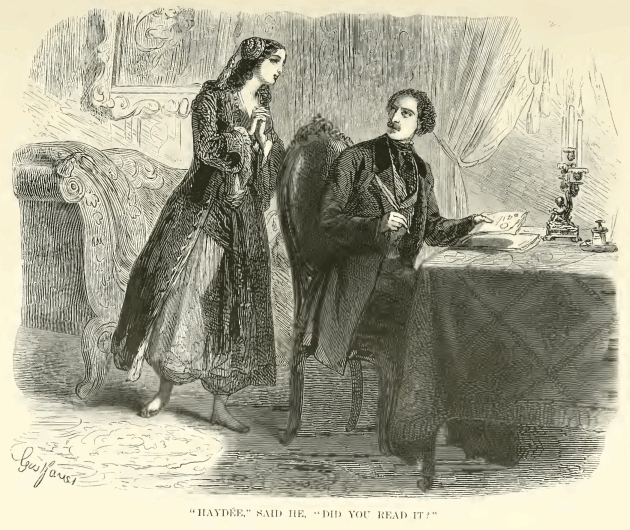
\includegraphics[width=\textwidth]{40241m.jpg}
\end{figure}

He was finishing the last line when a cry behind him made him start,
and the pen fell from his hand.

“Haydée,” said he, “did you read it?”

“Oh, my lord,” said she, “why are you writing thus at such an hour? Why
are you bequeathing all your fortune to me? Are you going to leave me?”

“I am going on a journey, dear child,” said Monte Cristo, with an
expression of infinite tenderness and melancholy; “and if any
misfortune should happen to me——”

The count stopped.

“Well?” asked the young girl, with an authoritative tone the count had
never observed before, and which startled him.

“Well, if any misfortune happen to me,” replied Monte Cristo, “I wish
my daughter to be happy.” Haydée smiled sorrowfully, and shook her
head.

“Do you think of dying, my lord?” said she.

“The wise man, my child, has said, ‘It is good to think of death.’”

“Well, if you die,” said she, “bequeath your fortune to others, for if
you die I shall require nothing;” and, taking the paper, she tore it in
four pieces, and threw it into the middle of the room. Then, the effort
having exhausted her strength, she fell, not asleep this time, but
fainting on the floor.

The count leaned over her and raised her in his arms; and seeing that
sweet pale face, those lovely eyes closed, that beautiful form
motionless and to all appearance lifeless, the idea occurred to him for
the first time, that perhaps she loved him otherwise than as a daughter
loves a father.

“Alas,” murmured he, with intense suffering, “I might, then, have been
happy yet.”

Then he carried Haydée to her room, resigned her to the care of her
attendants, and returning to his study, which he shut quickly this
time, he again copied the destroyed will. As he was finishing, the
sound of a cabriolet entering the yard was heard. Monte Cristo
approached the window, and saw Maximilian and Emmanuel alight. “Good,”
said he; “it was time,”—and he sealed his will with three seals.

A moment afterwards he heard a noise in the drawing-room, and went to
open the door himself. Morrel was there; he had come twenty minutes
before the time appointed.

“I am perhaps come too soon, count,” said he, “but I frankly
acknowledge that I have not closed my eyes all night, nor has anyone in
my house. I need to see you strong in your courageous assurance, to
recover myself.”

Monte Cristo could not resist this proof of affection; he not only
extended his hand to the young man, but flew to him with open arms.

“Morrel,” said he, “it is a happy day for me, to feel that I am beloved
by such a man as you. Good-morning, Emmanuel; you will come with me
then, Maximilian?”

“Did you doubt it?” said the young captain.

“But if I were wrong——”

“I watched you during the whole scene of that challenge yesterday; I
have been thinking of your firmness all night, and I said to myself
that justice must be on your side, or man’s countenance is no longer to
be relied on.”

“But, Morrel, Albert is your friend?”

“Simply an acquaintance, sir.”

“You met on the same day you first saw me?”

“Yes, that is true; but I should not have recollected it if you had not
reminded me.”

“Thank you, Morrel.” Then ringing the bell once, “Look.” said he to
Ali, who came immediately, “take that to my solicitor. It is my will,
Morrel. When I am dead, you will go and examine it.”

“What?” said Morrel, “you dead?”

“Yes; must I not be prepared for everything, dear friend? But what did
you do yesterday after you left me?”

“I went to Tortoni’s, where, as I expected, I found Beauchamp and
Château-Renaud. I own I was seeking them.”

“Why, when all was arranged?”

“Listen, count; the affair is serious and unavoidable.”

“Did you doubt it!”

“No; the offence was public, and everyone is already talking of it.”

“Well?”

“Well, I hoped to get an exchange of arms,—to substitute the sword for
the pistol; the pistol is blind.”

“Have you succeeded?” asked Monte Cristo quickly, with an imperceptible
gleam of hope.

“No; for your skill with the sword is so well known.”

“Ah?—who has betrayed me?”

“The skilful swordsman whom you have conquered.”

“And you failed?”

“They positively refused.”

“Morrel,” said the count, “have you ever seen me fire a pistol?”

“Never.”

“Well, we have time; look.” Monte Cristo took the pistols he held in
his hand when Mercédès entered, and fixing an ace of clubs against the
iron plate, with four shots he successively shot off the four sides of
the club. At each shot Morrel turned pale. He examined the bullets with
which Monte Cristo performed this dexterous feat, and saw that they
were no larger than buckshot.

“It is astonishing,” said he. “Look, Emmanuel.” Then turning towards
Monte Cristo, “Count,” said he, “in the name of all that is dear to
you, I entreat you not to kill Albert!—the unhappy youth has a mother.”

“You are right,” said Monte Cristo; “and I have none.” These words were
uttered in a tone which made Morrel shudder.

“You are the offended party, count.”

“Doubtless; what does that imply?”

“That you will fire first.”

“I fire first?”

“Oh, I obtained, or rather claimed that; we had conceded enough for
them to yield us that.”

“And at what distance?”

“Twenty paces.” A smile of terrible import passed over the count’s
lips.

“Morrel,” said he, “do not forget what you have just seen.”

“The only chance for Albert’s safety, then, will arise from your
emotion.”

“I suffer from emotion?” said Monte Cristo.

“Or from your generosity, my friend; to so good a marksman as you are,
I may say what would appear absurd to another.”

“What is that?”

“Break his arm—wound him—but do not kill him.”

“I will tell you, Morrel,” said the count, “that I do not need
entreating to spare the life of M. de Morcerf; he shall be so well
spared, that he will return quietly with his two friends, while I——”

“And you?”

“That will be another thing; I shall be brought home.”

“No, no,” cried Maximilian, quite unable to restrain his feelings.

“As I told you, my dear Morrel, M. de Morcerf will kill me.”

Morrel looked at him in utter amazement. “But what has happened, then,
since last evening, count?”

“The same thing that happened to Brutus the night before the battle of
Philippi; I have seen a ghost.”

“And that ghost——”

“Told me, Morrel, that I had lived long enough.”

Maximilian and Emmanuel looked at each other. Monte Cristo drew out his
watch. “Let us go,” said he; “it is five minutes past seven, and the
appointment was for eight o’clock.”

A carriage was in readiness at the door. Monte Cristo stepped into it
with his two friends. He had stopped a moment in the passage to listen
at a door, and Maximilian and Emmanuel, who had considerately passed
forward a few steps, thought they heard him answer by a sigh to a sob
from within. As the clock struck eight they drove up to the place of
meeting.

“We are first,” said Morrel, looking out of the window.

“Excuse me, sir,” said Baptistin, who had followed his master with
indescribable terror, “but I think I see a carriage down there under
the trees.”

Monte Cristo sprang lightly from the carriage, and offered his hand to
assist Emmanuel and Maximilian. The latter retained the count’s hand
between his.

“I like,” said he, “to feel a hand like this, when its owner relies on
the goodness of his cause.”

“It seems to me,” said Emmanuel, “that I see two young men down there,
who are evidently, waiting.”

Monte Cristo drew Morrel a step or two behind his brother-in-law.

“Maximilian,” said he, “are your affections disengaged?” Morrel looked
at Monte Cristo with astonishment. “I do not seek your confidence, my
dear friend. I only ask you a simple question; answer it;—that is all I
require.”

“I love a young girl, count.”

“Do you love her much?”

“More than my life.”

“Another hope defeated!” said the count. Then, with a sigh, “Poor
Haydée!” murmured he.

“To tell the truth, count, if I knew less of you, I should think that
you were less brave than you are.”

“Because I sigh when thinking of someone I am leaving? Come, Morrel, it
is not like a soldier to be so bad a judge of courage. Do I regret
life? What is it to me, who have passed twenty years between life and
death? Moreover, do not alarm yourself, Morrel; this weakness, if it is
such, is betrayed to you alone. I know the world is a drawing-room,
from which we must retire politely and honestly; that is, with a bow,
and our debts of honor paid.”

“That is to the purpose. Have you brought your arms?”

“I?—what for? I hope these gentlemen have theirs.”

“I will inquire,” said Morrel.

“Do; but make no treaty—you understand me?”

“You need not fear.” Morrel advanced towards Beauchamp and
Château-Renaud, who, seeing his intention, came to meet him. The three
young men bowed to each other courteously, if not affably.

“Excuse me, gentlemen,” said Morrel, “but I do not see M. de Morcerf.”

“He sent us word this morning,” replied Château-Renaud, “that he would
meet us on the ground.”

“Ah,” said Morrel. Beauchamp pulled out his watch.

“It is only five minutes past eight,” said he to Morrel; “there is not
much time lost yet.”

“Oh, I made no allusion of that kind,” replied Morrel.

“There is a carriage coming,” said Château-Renaud. It advanced rapidly
along one of the avenues leading towards the open space where they were
assembled.

“You are doubtless provided with pistols, gentlemen? M. de Monte Cristo
yields his right of using his.”

“We had anticipated this kindness on the part of the count,” said
Beauchamp, “and I have brought some weapons which I bought eight or ten
days since, thinking to want them on a similar occasion. They are quite
new, and have not yet been used. Will you examine them.”

“Oh, M. Beauchamp, if you assure me that M. de Morcerf does not know
these pistols, you may readily believe that your word will be quite
sufficient.”

“Gentlemen,” said Château-Renaud, “it is not Morcerf coming in that
carriage;—faith, it is Franz and Debray!”

The two young men he announced were indeed approaching. “What chance
brings you here, gentlemen?” said Château-Renaud, shaking hands with
each of them.

“Because,” said Debray, “Albert sent this morning to request us to
come.” Beauchamp and Château-Renaud exchanged looks of astonishment. “I
think I understand his reason,” said Morrel.

“What is it?”

“Yesterday afternoon I received a letter from M. de Morcerf, begging me
to attend the Opera.”

“And I,” said Debray.

“And I also,” said Franz.

“And we, too,” added Beauchamp and Château-Renaud.

“Having wished you all to witness the challenge, he now wishes you to
be present at the combat.”

“Exactly so,” said the young men; “you have probably guessed right.”

“But, after all these arrangements, he does not come himself,” said
Château-Renaud. “Albert is ten minutes after time.”

“There he comes,” said Beauchamp, “on horseback, at full gallop,
followed by a servant.”

“How imprudent,” said Château-Renaud, “to come on horseback to fight a
duel with pistols, after all the instructions I had given him.”

“And besides,” said Beauchamp, “with a collar above his cravat, an open
coat and white waistcoat! Why has he not painted a spot upon his
heart?—it would have been more simple.”

Meanwhile Albert had arrived within ten paces of the group formed by
the five young men. He jumped from his horse, threw the bridle on his
servant’s arms, and joined them. He was pale, and his eyes were red and
swollen; it was evident that he had not slept. A shade of melancholy
gravity overspread his countenance, which was not natural to him.

“I thank you, gentlemen,” said he, “for having complied with my
request; I feel extremely grateful for this mark of friendship.” Morrel
had stepped back as Morcerf approached, and remained at a short
distance. “And to you also, M. Morrel, my thanks are due. Come, there
cannot be too many.”

\begin{figure}[ht]
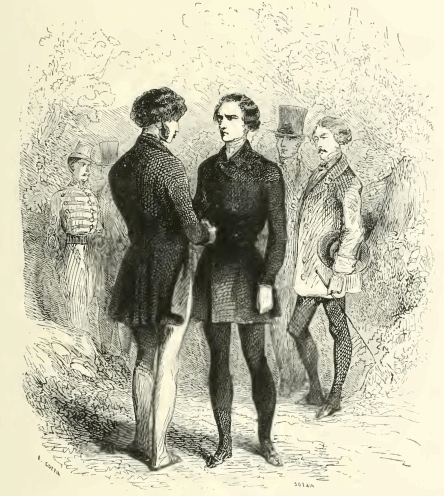
\includegraphics[width=\textwidth]{40248m.jpg}
\end{figure}

“Sir,” said Maximilian, “you are not perhaps aware that I am M. de
Monte Cristo’s friend?”

“I was not sure, but I thought it might be so. So much the better; the
more honorable men there are here the better I shall be satisfied.”

“M. Morrel,” said Château-Renaud, “will you apprise the Count of Monte
Cristo that M. de Morcerf is arrived, and we are at his disposal?”

Morrel was preparing to fulfil his commission. Beauchamp had meanwhile
drawn the box of pistols from the carriage.

“Stop, gentlemen,” said Albert; “I have two words to say to the Count
of Monte Cristo.”

“In private?” asked Morrel.

“No, sir; before all who are here.”

Albert’s witnesses looked at each other. Franz and Debray exchanged
some words in a whisper, and Morrel, rejoiced at this unexpected
incident, went to fetch the count, who was walking in a retired path
with Emmanuel.

“What does he want with me?” said Monte Cristo.

“I do not know, but he wishes to speak to you.”

“Ah?” said Monte Cristo, “I trust he is not going to tempt me by some
fresh insult!”

“I do not think that such is his intention,” said Morrel.

The count advanced, accompanied by Maximilian and Emmanuel. His calm
and serene look formed a singular contrast to Albert’s grief-stricken
face, who approached also, followed by the other four young men.

When at three paces distant from each other, Albert and the count
stopped.

“Approach, gentlemen,” said Albert; “I wish you not to lose one word of
what I am about to have the honor of saying to the Count of Monte
Cristo, for it must be repeated by you to all who will listen to it,
strange as it may appear to you.”

“Proceed, sir,” said the count.

“Sir,” said Albert, at first with a tremulous voice, but which
gradually became firmer, “I reproached you with exposing the conduct of
M. de Morcerf in Epirus, for guilty as I knew he was, I thought you had
no right to punish him; but I have since learned that you had that
right. It is not Fernand Mondego’s treachery towards Ali Pasha which
induces me so readily to excuse you, but the treachery of the fisherman
Fernand towards you, and the almost unheard-of miseries which were its
consequences; and I say, and proclaim it publicly, that you were
justified in revenging yourself on my father, and I, his son, thank you
for not using greater severity.”

Had a thunderbolt fallen in the midst of the spectators of this
unexpected scene, it would not have surprised them more than did
Albert’s declaration. As for Monte Cristo, his eyes slowly rose towards
heaven with an expression of infinite gratitude. He could not
understand how Albert’s fiery nature, of which he had seen so much
among the Roman bandits, had suddenly stooped to this humiliation. He
recognized the influence of Mercédès, and saw why her noble heart had
not opposed the sacrifice she knew beforehand would be useless.

“Now, sir,” said Albert, “if you think my apology sufficient, pray give
me your hand. Next to the merit of infallibility which you appear to
possess, I rank that of candidly acknowledging a fault. But this
confession concerns me only. I acted well as a man, but you have acted
better than man. An angel alone could have saved one of us from
death—that angel came from heaven, if not to make us friends (which,
alas, fatality renders impossible), at least to make us esteem each
other.”

Monte Cristo, with moistened eye, heaving breast, and lips half open,
extended to Albert a hand which the latter pressed with a sentiment
resembling respectful fear.

“Gentlemen,” said he, “M. de Monte Cristo receives my apology. I had
acted hastily towards him. Hasty actions are generally bad ones. Now my
fault is repaired. I hope the world will not call me cowardly for
acting as my conscience dictated. But if anyone should entertain a
false opinion of me,” added he, drawing himself up as if he would
challenge both friends and enemies, “I shall endeavor to correct his
mistake.”

“What happened during the night?” asked Beauchamp of Château-Renaud;
“we appear to make a very sorry figure here.”

“In truth, what Albert has just done is either very despicable or very
noble,” replied the baron.

“What can it mean?” said Debray to Franz.

“The Count of Monte Cristo acts dishonorably to M. de Morcerf, and is
justified by his son! Had I ten Yaninas in my family, I should only
consider myself the more bound to fight ten times.”

As for Monte Cristo, his head was bent down, his arms were powerless.
Bowing under the weight of twenty-four years’ reminiscences, he thought
not of Albert, of Beauchamp, of Château-Renaud, or of any of that
group; but he thought of that courageous woman who had come to plead
for her son’s life, to whom he had offered his, and who had now saved
it by the revelation of a dreadful family secret, capable of destroying
forever in that young man’s heart every feeling of filial piety.

“Providence still,” murmured he; “now only am I fully convinced of
being the emissary of God!”
